% Analyze Boulder Meetup
% 2013-06-05 
% Josh Montague, Data Scientist @Gnip
% @jrmontag

\documentclass{beamer}
\setbeamertemplate{navigation symbols}{}
\usetheme{gnip}

% packages
\usepackage{siunitx}
\usepackage{graphicx}
\usepackage{hyperref}
\usepackage[absolute,overlay]{textpos}
  \setlength{\TPHorizModule}{1mm}
  \setlength{\TPVertModule}{1mm}
%\usepackage{fontspec}			%requires different tex engine
%\usepackage{minted}			%highlighted source code
%\usepackage{tikz}				%programatic graphic creation

% footer
\setbeamertemplate{footline}[text line]{
\colorbox{white}{\parbox[25px]{\paperwidth} {\color{linecolour} {\line(1,0){500} \\ \hfill @jrmontag -- @Gnip}}}}
\beamersetuncovermixins{\opaqueness<1>{25}}{\opaqueness<2->{15}}

% title info
\title{Data Science @ Gnip }
\subtitle{\emph{\#AnalyzeBoulder} Meetup}
\author{Josh Montague\texorpdfstring{\\ Data Scientist, Gnip Inc. \\ @jrmontag}{}} 
\date{\today} 
% beamer doesn't like \\ breaks in this context. above hack via http://tex.stackexchange.com/questions/10555/hyperref-warning-token-not-allowed-in-a-pdf-string


\begin{document}


%%%%%%%%%%%%%%%%%% title %%%%%%%%%%%%%%%%%%%
\begin{frame}
\titlepage
\end{frame}


%%%%%%%%%%%%%%%%%% gnip (quick facts) %%%%%%%%%%%%%%%%%%%
\begin{frame} \frametitle{Gnip}

\vspace{0.2in}

\LARGE{Where $\to$  \hspace{0.55in} Here! (Boulder, CO) }

\vspace{0.2in}

\LARGE{Who $\to  \hspace{1.2in} \approx$ 60 people* } 

\vspace{0.2in}

\LARGE{What $\to$ \hspace{0.7in} social data provider}

\vspace{0.7in}

% cheap way to right-justify
{\hfill \Large{*and hiring!}} 

{\hfill \normalsize\url{http://gnip.com/careers}}
\end{frame}


%%%%%%%%%%%%%%%%%% gnip (data sources) %%%%%%%%%%%%%%%%%%%
\begin{frame} \frametitle{sources \& volumes}

\vspace{0.1in}

\begin{table}
	\begin{tabular}{l|r}
		\hline
		{Publisher$^\dagger$}			&   	{Daily Activities} \\
		\hline 
		Twitter      					&	500 M \\
		Tumblr      					&	90 M \\
		Foursquare      					&	5 M \\
		Disqus       					&	1.7 M \\
		Wordpress$^{a}$ Comments 		&	1.7 M \\
		Wordpress$^{a}$ Posts 			&	1 M \\
		`Engagement'$^{b}$ 			&	2.4 M \\
		\hline
	\end{tabular}
\end{table}
% footnotes
$^a$.com + .org \\
$^b$ likes, votes (Disqus, WP, Tumblr, IntenseDebate) \\

{\tiny
$^\dagger$Add'l Premium Publishers: StockTwits, Newsgator; EDC Streams: Facebook, YouTube, Google+, flickr, bitly, Dailymotion, Delicious, Identi.ca, Instagram. Metacafe, Panoramio, Photobucket, Plurk, Reddit, StackOverflow, Vimeo
}

\begin{center}
	\LARGE{\emph{4 B activities delivered daily}}
\end{center}

\end{frame}


%%%%%%%%%%%%%%%%%% data science team %%%%%%%%%%%%%%%%%%%
\begin{frame} \frametitle{our team}

3.5 data scientists (academic backgrounds)

\vspace{0.3in}

`marketing'  $\to$ 3x roles: marketing + sales + product

\vspace{0.3in}

ask Qs, answer Qs (about our data)

\end{frame}


%%%%%%%%%%%%%%%%%%% social data v social media %%%%%%%%%%%%%%%%%%%
% use image as slide background
%{
%\usebackgroundtemplate{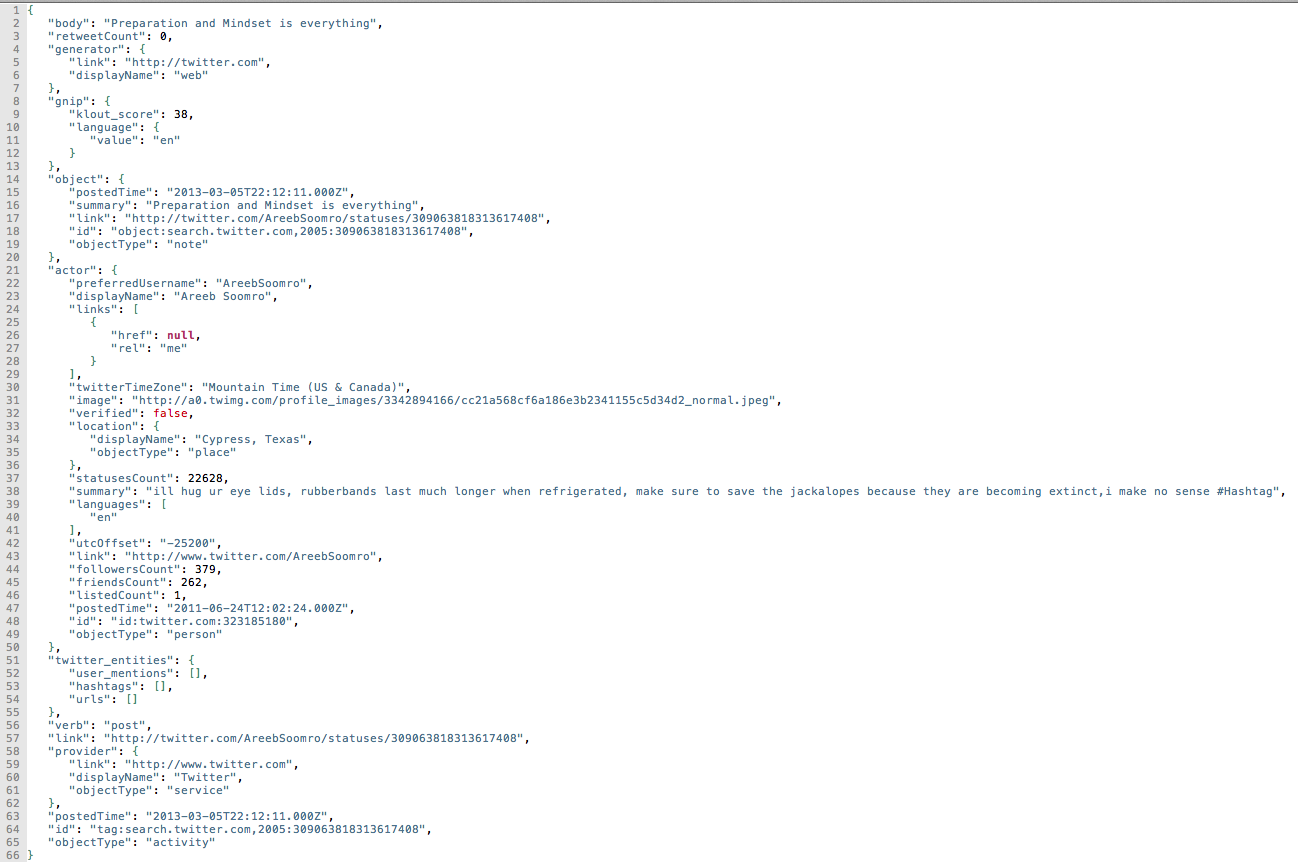
\includegraphics[width=\paperwidth]{./imgs/twac.png}}
%
%\begin{frame} \frametitle{\textcolor{black} {social data (v. media)}}
%
%%\begin{textblock}{40}(65,60)		%bottom right
%\begin{textblock}{40}(75,12)		%top right
%	
\includegraphics[scale=0.25]{./imgs/tweet.png}
%\end{textblock}
%
%\end{frame}
%}


%%%%%%%%%%%%%%%%%% social data v social media %%%%%%%%%%%%%%%%%%%
\begin{frame} \frametitle{\textcolor{white} {social data (v. media)}}

\begin{textblock}{1}(1,12)
	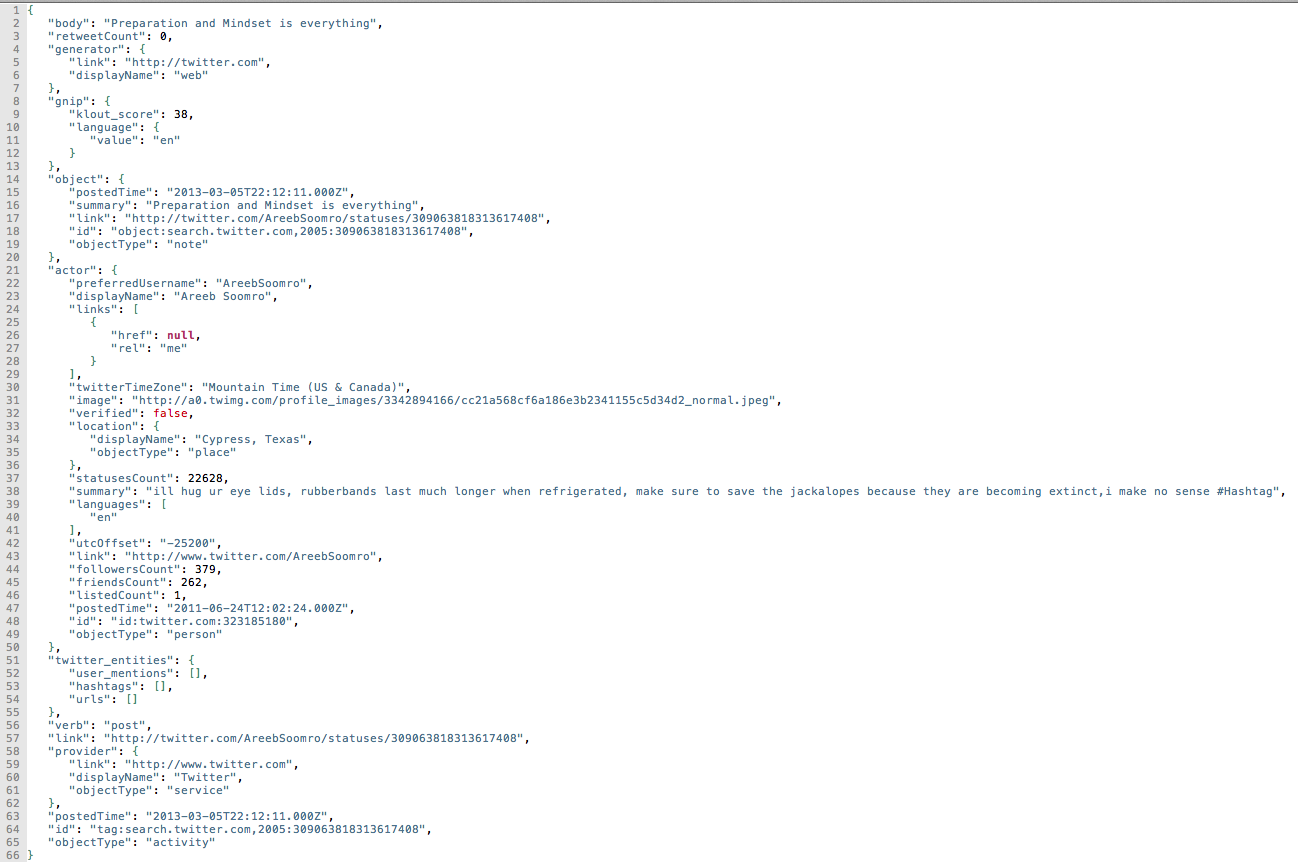
\includegraphics[scale=0.26]{./imgs/twac.png}
\end{textblock}

%\begin{textblock}{40}(65,60)		%bottom right
\begin{textblock}{40}(62,15)		%top right
	
\includegraphics[scale=0.25]{./imgs/tweet.png}
\end{textblock}

\end{frame}


%%%%%%%%%%%%%%%%%% project: disqus %%%%%%%%%%%%%%%%%%%
\begin{frame} \frametitle{ex: Disqus comment threads}

\begin{textblock}{1}(5,15)
	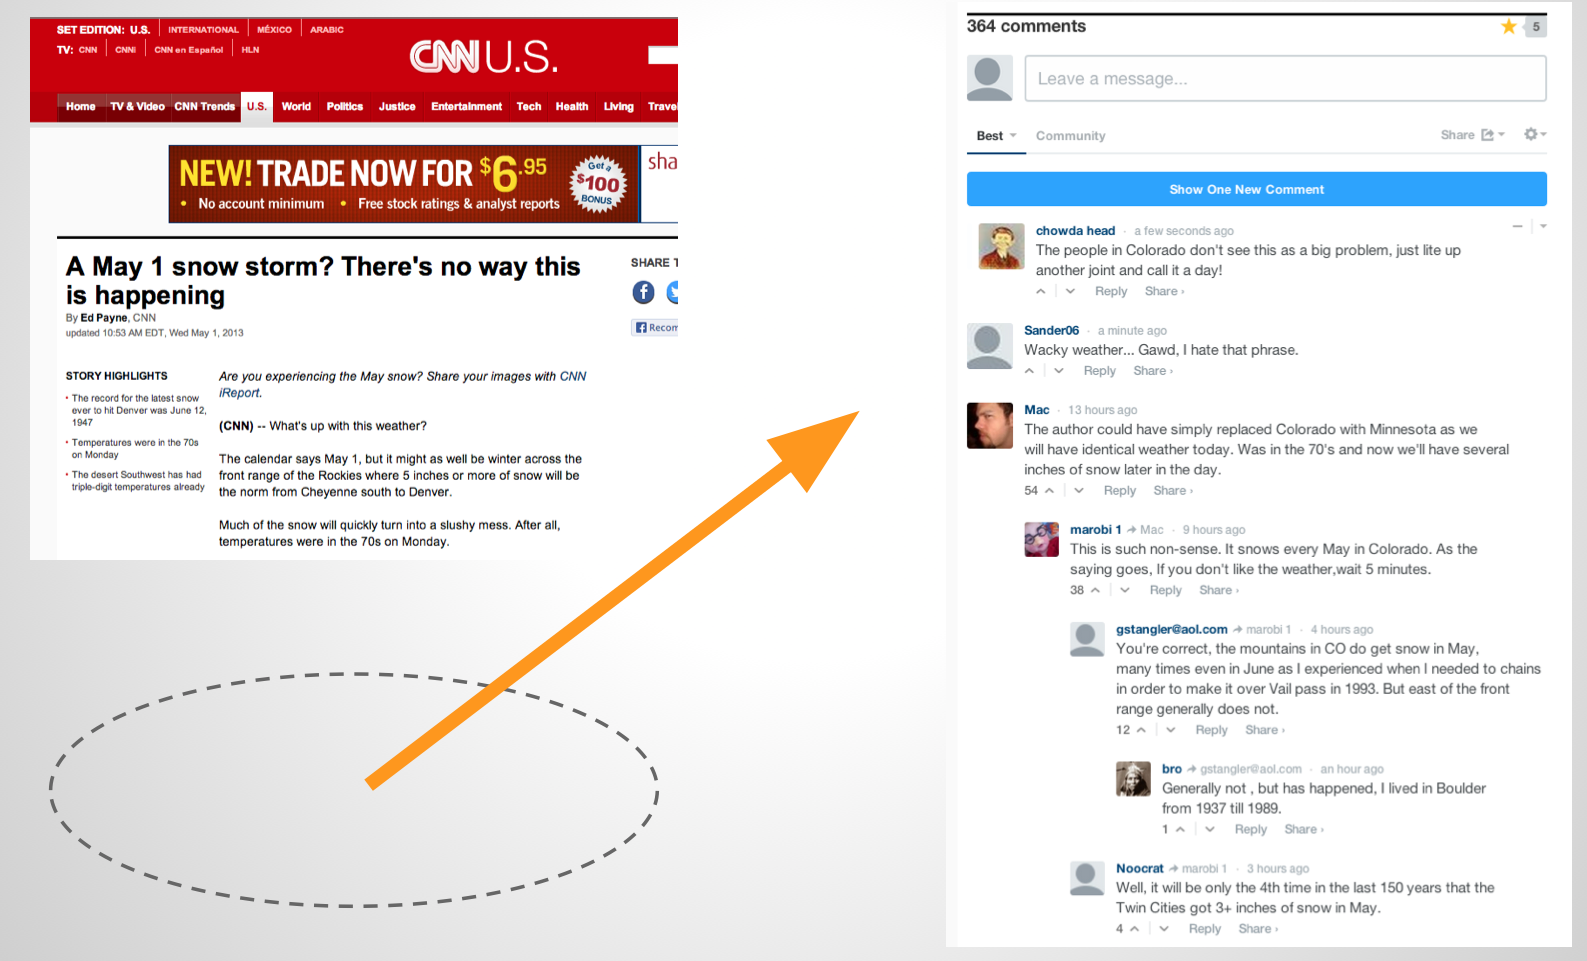
\includegraphics[scale=0.21]{./imgs/disqus1.png}
\end{textblock}

\end{frame}

%
\begin{frame} \frametitle{ex: Disqus comment threads}

\begin{textblock}{1}(5,15)
	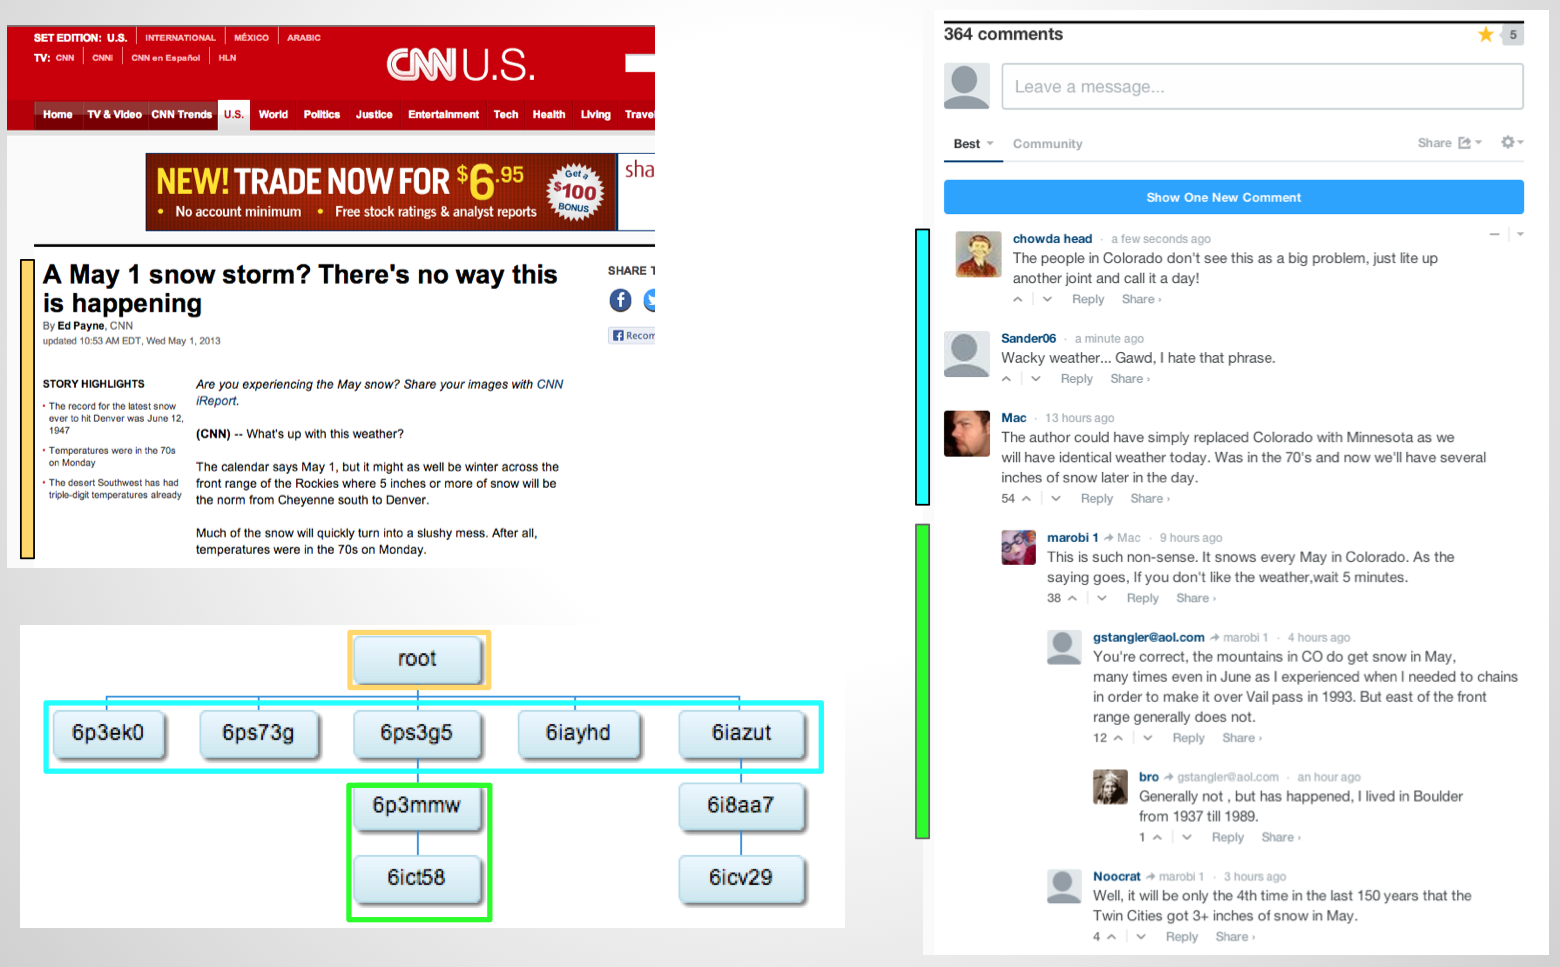
\includegraphics[scale=0.21]{./imgs/disqus3.png}
\end{textblock}

\end{frame}

%
\begin{frame} \frametitle{ex: Disqus comment threads}

\begin{textblock}{1}(1,14)
	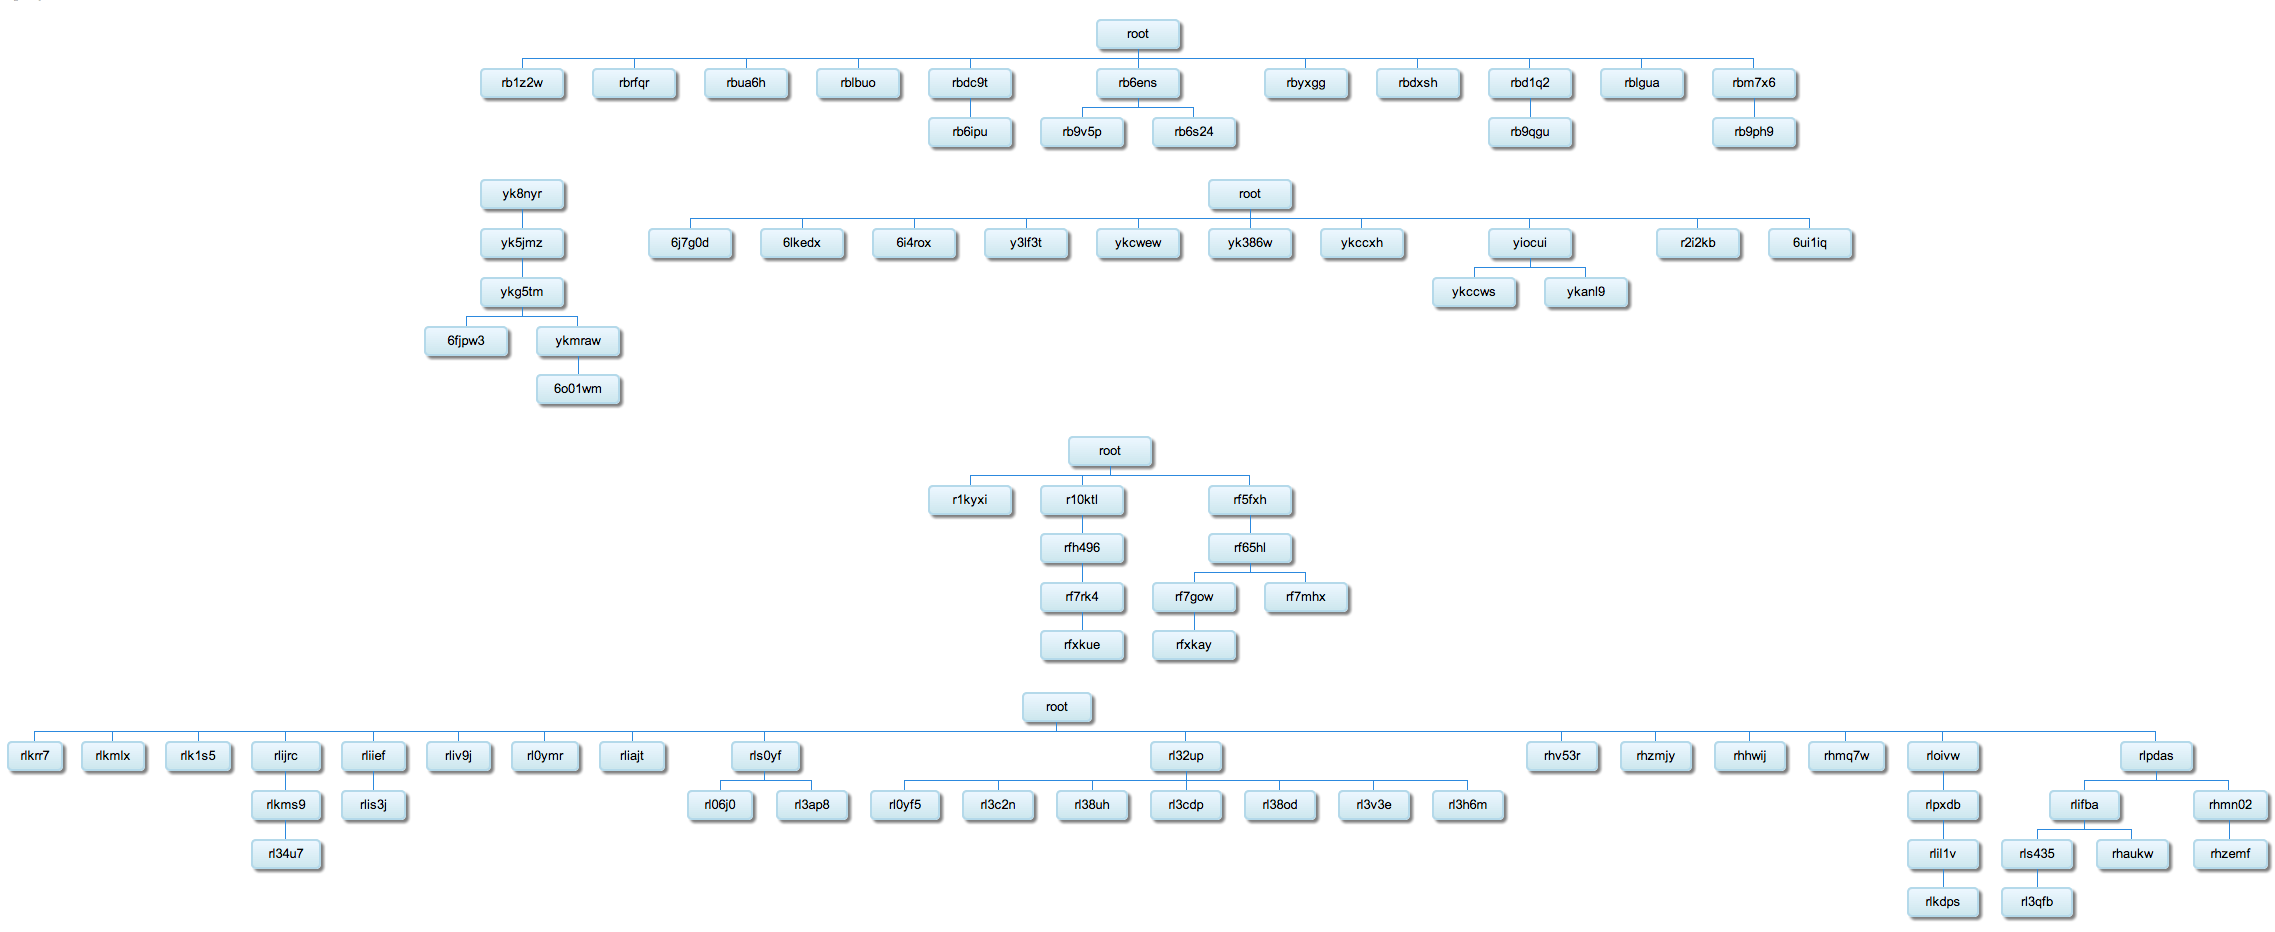
\includegraphics[scale=0.155]{./imgs/disqus4.png}
\end{textblock}

\begin{textblock}{1}(14,67)
	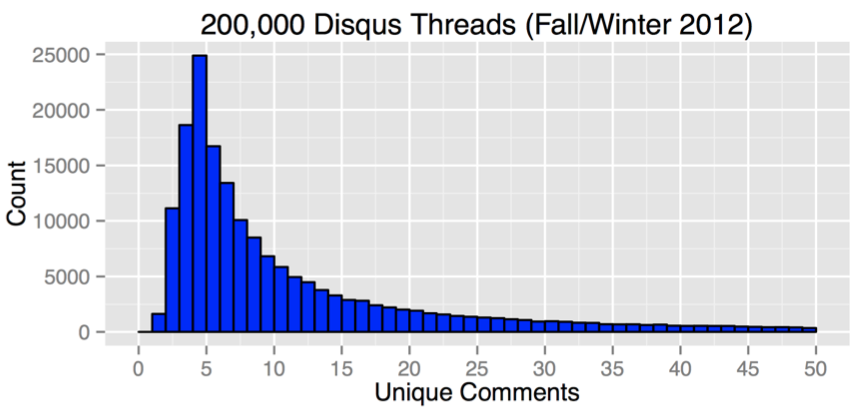
\includegraphics[scale=0.165]{./imgs/disqus5.png}
\end{textblock}

\begin{textblock}{1}(66,67)
	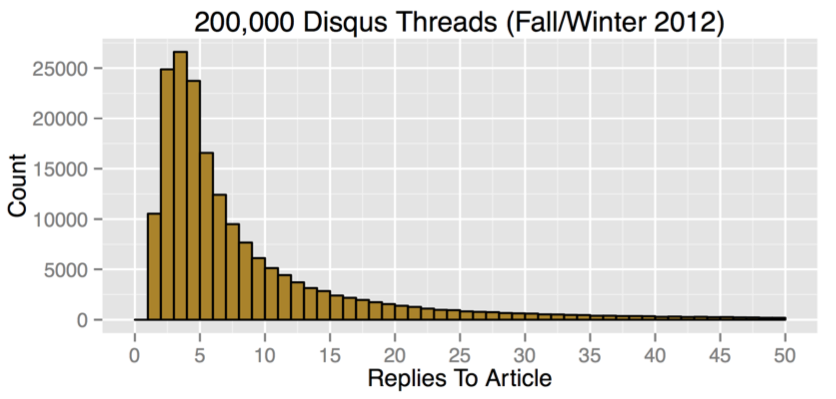
\includegraphics[scale=0.17]{./imgs/disqus6.png}
\end{textblock}

\end{frame}


%%%%%%%%%%%%%%%%%% the end %%%%%%%%%%%%%%%%%%%
\begin{frame} \frametitle{}

\vspace{0.5in}

\begin{center}
\Huge{thanks!}

\vspace{0.5in}

\normalsize{source/slides: \\
\url{http://bit.ly/ABMeetup}}

\vspace{0.5in}

\Large{Don't forget, we're hiring!} \\
\url{http://gnip.com/careers}
\end{center}

\end{frame}

\end{document}
